\documentclass{article}
\usepackage[utf8]{inputenc}
\usepackage{amssymb}
\usepackage{tikz}
\usepackage{amsmath}
\usepackage{relsize}
\usepackage{mathtools}
\usepackage{textcomp}
\usepackage{eurosym}
\usepackage{amssymb}
\usepackage{systeme}
\usepackage{mathtools}
\usepackage{graphicx}
\usepackage{subfig}
\usepackage[bottom]{footmisc}
\usepackage{mwe}
\usepackage{csquotes}
\usepackage[colorinlistoftodos]{todonotes}
\usepackage{subfig}
\usepackage{color,soul}

\title{Method}
\author{Roman Oort}
\date{\today}

%%% PERSONAL SHORTCUTS
\DeclareMathOperator*{\plim}{plim}
\newcommand{\T}{\textbf{T}}
\newcommand{\Tij}{\textbf{T}_{ij}}
\newcommand{\Soc}{(\T(n))^{\infty}_{n=1}}
\newcommand{\beli}[3][2]{p_{#2}^{(#3)}}
\newcommand{\belvec}[2]{\textbf{p}^{(#2)}}

\begin{document}

\maketitle

\tableofcontents
\newpage

\section{Network Generation}

\subsection{Random Generation}
\label{generation:random}
In order to allow for proper analysis of the DeGroot mechanics a method to generate \emph{random} networks was created, to ensure generality of the obtained results. Given a number of agents this method is capable of generating both directed and undirected networks, and accepts several other parameters to shape the generation as desired.

\subsubsection{Default Case}
In the default, most basic, case this function simply takes the desired number of agents, $n$ as input. Other, optional, parameters can be provided to customize the desired network and will be discussed in detail at the relevant time.
To start, an empty $n\times n$ array \cite{2020NumPy-Array}, i.e. containing solely zeroes, is created, which serves as a blank slate for the interaction matrix $\T$ of the network\hl{, which is all that is required to describe a network as discussed in [REF].}\todo{Possibly unnecessary}
Subsequently the function will iteratively add the links for every agent in the network, in order to ensure the generated network is fully connected at every size. \newline
In this iteration there is one special case, namely, the very first agent. To ensure aperiodicity, as discussed in [REF], and therefore convergence, the very first agent is guaranteed to receive a self-link. As this creates a cycle of length one, aperiodicity is guaranteed. \newline

Every subsequent agent, when generating a directed network, will be guaranteed to both receive and send one link. When generating an undirected network each agent is guaranteed to have one link, which is both incoming and outgoing. This guarantees that the network of size $n$ will be fully connected. However, as the interest lies in sequences of networks, all of which need to be convergent, this condition needs to be met by every network in the sequence of size $n^{\prime} < n$, not only by the network of size $n$. Therefore, these guaranteed links will be sent to, and by, an earlier agent in the network, that is to say that the guaranteed links of an agent $k$ can only be sent to and received by any agent $m < k$. This guarantees the strong connectedness of the network, at every size, which can be proven inductively [REF]. This also holds for an undirected network, where the only difference is that the agents receiving and sending a link are one and the same. The specific agents on the other end of these guaranteed links are sampled randomly from a uniform distribution over the interval of agents already present in the network. \newline

Therefore, as this method of generation not only guarantees connectedness in the total network, but also at every smaller size of the network, this returned network can also be considered a sequence of networks. To access a network of a specific size in this sequence, one would only need to take the rows and columns up to that size to obtain the specific network. This ensures that the network and its links stay constant between sizes, allowing for proper comparison of different networks in the sequence. Finally, this function is also capable of growing an existing network: when a matrix and a positive integer $m$ are provided, the function will grow this existing matrix by adding $m$ rows and columns, one for each agent, whose links are determined in the same way as described earlier.\newline

This method of generating these network was chosen over more standard methods of model generation for several reasons. For starters, implementing the network generation from scratch provides more low-level control over the network generation process, allowing more options for customization. A clear effect is the strong connectedness mentioned earlier. Using another method for generating the network, while possibly faster when initially generating the network, would require another pass over all agents to ensure the network is fully connected, and remains so at every size. 

Another, more subtle, effect of the chosen method is a slight bias towards the earlier agents in the network, an effect which can be seen in figure (\ref{degree:agent}) below, which shows the average degree for each consecutive 100 agents. As shown earlier the agents are added to the network the higher their degree tends to be. This mirrors how those individuals who are part of a group for a long time tend to have more connection than those new to the group.

\begin{center}
    \begin{figure}[!htbp]
        \centering
        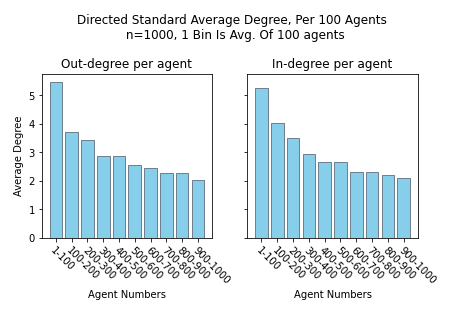
\includegraphics[width=.8\textwidth]{ThesisKI/Images/DirectedStandardPerAgent.png}
        \caption{Average Degree per 100 agents}
        \label{degree:agent}
    \end{figure}
\end{center}
\newpage
\subsubsection{Customization}

As mentioned the chosen implementation has the option to adjust the generation process as desired. These adjustment are applied complementary to the default generation, to ensure the base guarantees of this method. \newline

First of all, this method allows for the generation of both directed and undirected networks. The method for generating undirected networks is very similar to the generation of directed networks. In fact, the process is entirely the same, save for one detail. In contrast to the generation of a directed network, where the agents to receive and send a link are chosen independently, and therefore tend to be distinct agents, the generation of an undirected network simply chooses one random agent to both receive and send a link. After all, the only difference between the interaction matrix $\T$ of a directed and undirected network is that the matrix of an undirected is symmetrical, whereas the matrix of an undirected network is asymmetrical. \newline
Furthermore, when a directed network is created it can be made into an undirected network. This is done by simply taking the element wise maximum between the original matrix and its transpose, effectively mirroring all links in the matrix along the diagonal. \newline

Secondly, there is also the option to increase the degree of the agents to more than the base minimum. Using the default generation results in 
\begin{figure}[!htbp]
  \centering
  \subfloat[Standard Degree]{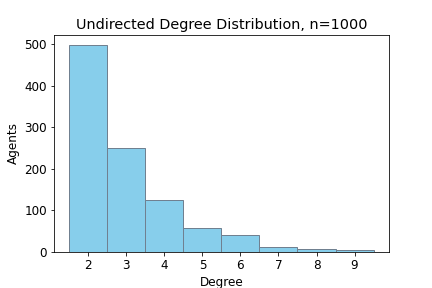
\includegraphics[width=0.5\textwidth]{ThesisKI/Images/DegreeUndirectedStd.png}\label{deg:std}}
  \hfill
  \subfloat[Increased Degree]{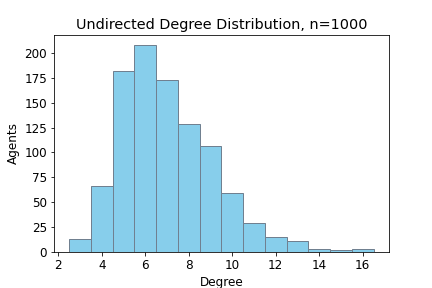
\includegraphics[width=0.5\textwidth]{ThesisKI/Images/DegreeUndirectedInc.png}\label{deg:inc}}
  \caption{Degree Distributions}
\end{figure}

\newpage

The implementation of this increased degree is rolled into the generation of the network to roll this functionality into the iteration of the generation function, preventing the need to repeat this iteration if the degree would be increased after the generation. After the guaranteed connections each agent then gets assigned an additional degree, which is a random number sampled from a given probability distribution, by default $\mathcal{N}(2,1)$. This number is rounded to the nearest integer. Subsequently, a corresponding amount of agents are drawn randomly from the set of \emph{all} agents in the network, and a link is created for those agents. When generating a directed network this procedure, including a random additional degree, occurs twice, once for the incoming degree, once for the outgoing degree. However, for an undirected network this procedure only needs to be executed once, and the chosen agents are used for both the incoming and outgoing link. \newline
The generation of this additional degree can customized further by providing a different probability function and the corresponding parameters. This allows for the degree to be increased as much as desired, using any probability distribution.\newline

Finally, the probability for self-links in the network can be set as desired. To guarantee that each agent in the network has a self-link this parameter can be set to 1 and, conversely, to ensure no agent \footnote{Except for the first agent, which always receives a self-link to ensure aperiodicity} has a self-link this parameter can simply be set to 0. Any value in between gives each agent that probability to receive a self-link.

Figure \ref{network:random} is an example of an undirected network generated using this method, with increased degree\footnote{Self-links not shown}:
\begin{center}
    \begin{figure}[!htbp]
        \centering
        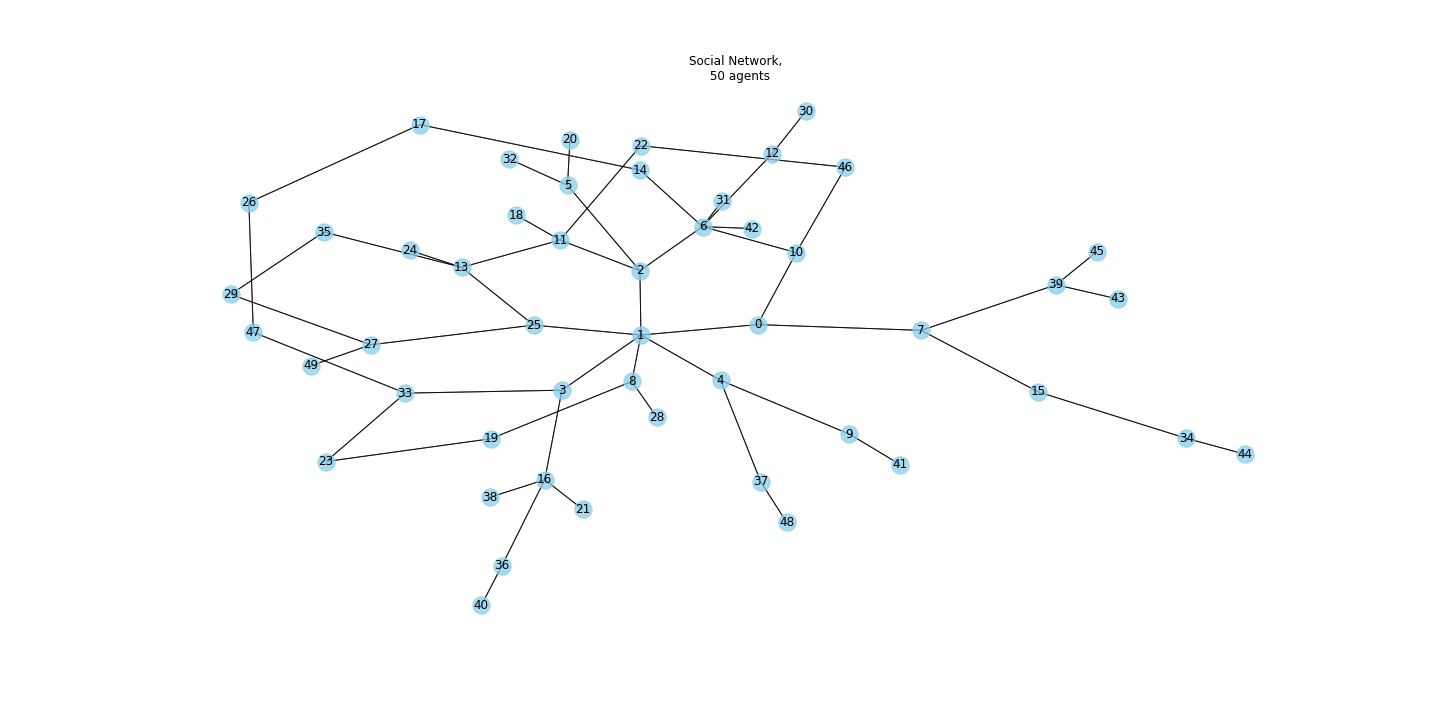
\includegraphics[width=1.1\textwidth]{ThesisKI/Images/NoneGraphRandom.png}
        \caption{Average Directed Degree}
        \label{network:random}
    \end{figure}
\end{center}

\newpage

\subsubsection{Sparse Matrices}

One caveat of the chosen method is the memory usage of matrices. As the interaction matrices are two-dimensional their memory usage increases quadratically as the network size increases. For small network this size this is negligible, however, as the sequences of networks grow towards the thousands of agents this becomes increasingly memory intensive. Therefore, in order to alleviate the intensive memory use of large matrices, the networks are generated as sparse matrices by default \cite{2020SciPy-NMeth}. As the generated network tend to contain only a small fraction of possible links the corresponding arrays will contain mainly zeros. However, it is not the lack of link that is of interest, but rather the presence of one, making all zero entries effectively a waste of space. Sparse matrices are created for this very purpose, increase memory efficiency of large arrays containing an overwhelming majority of empty data. The difference in memory usage is highlighted in figure \ref{generation:memory} below.

\begin{figure}[!htbp]
    \centering
    \subfloat[]{\label{generation:memory}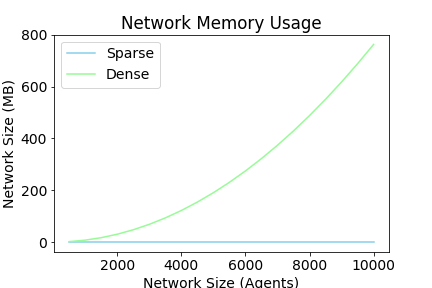
\includegraphics[scale=.45]{ThesisKI/Images/Memory.png}}
    
    \begin{minipage}{.5\linewidth}
    \centering
    \subfloat[]{\label{generation:time_inc}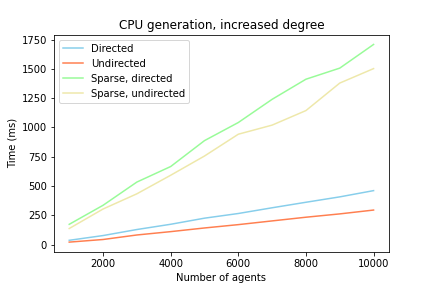
\includegraphics[scale=.4]{ThesisKI/Images/CPU_inc.png}}
    \end{minipage}%
    \begin{minipage}{.5\linewidth}
    \centering
    \subfloat[]{\label{generation:time_std}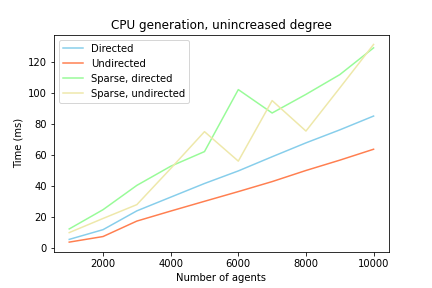
\includegraphics[scale=.4]{ThesisKI/Images/CPU.png}}
    \end{minipage}\par\medskip
    \caption{Network generation, \\ memory and time consumption}
\end{figure}

\newpage

While it is clear from the visualizations that the memory usage of sparse matrices, in this context, is an incredible improvement, it is not entirely without its downsides. As can be seen in figures \ref{generation:time_inc} and \ref{generation:time_std} sparse networks are slower to generate then their dense counterparts. However, the generation time for \emph{both} types still only increases linearly. As the generation time is only a one-time operation this difference can be considered negligible, making generation of networks using sparse networks the most beneficial default option.

\subsection{Fixed Generation}

\section{Belief Initialization}

The method to generate the beliefs of each agent works somewhat similar as the generation of the network itself. It can either be given a number of agents, $n$, for which to generate beliefs, or a pre-existing belief vector and a number of agents by which to grow it. The basis of the generation process is the same as described in [REF]. \newline
To start an array of $n$ random, zero mean, error terms, $e_i$, is generated, sampled from $\mathcal{N}(0, .75)$ by default. Then the assumed truth of the network $\mu$, which has been sampled from a uniform distribution over $[0, 1]$ at the initial generation of the network, is added to every term. \newline
However, there is one caveat to the belief generation as described above, namely that the beliefs are to lie on the interval $[0, 1]$. While $\mu$ does indeed lie on this interval, there is no guarantee that the initial beliefs, when generated as described, will too, as it is entirely possible for error terms to be generated that, when summed with $\mu$, will lie outside this interval. \newline
An initial instinct to would be to simply truncate the generated beliefs, i.e.: whenever the a generated belief exceeds this interval simply set it equal to the closest of either $0$ or $1$. However, as $\mu$ is drawn randomly it can lie arbitrarily close to either of the borders of the interval, which would ensure an unbalanced truncation to one side of the interval, which would cause the mean of the beliefs to shift away from $\mu$, disrupting convergence.\newline
Therefore, instead of truncating specific beliefs, the entire belief vector was normalized to lie on the interval $[0, 1]$, as follows:
\begin{equation*}
    \beli{i, \text{norm}}{0} = \frac{\beli{i}{0} - \min(\textbf{p}^{(0)})}{\max(\textbf{p}^{(0)}) - \min(\textbf{p}^{(0)})}
\end{equation*}

This ensures that none of the initial beliefs will exceed this threshold. Another solution to this problem would be to simply always set $\mu$ to $0.5$ and simply use a uniform distribution on the interval $[-0.5, 0.5]$ to sample the noise terms. However, this limits the choice of probability distributions of the error terms. This alternative method would always require the use of the uniform, or some other bounded distribution, to sample the noise terms. However, with the chosen method any probability function can be used, without any bounds.

\section{Weight Initialization}

While the network generation does create the links between agents and form the structure of the network, it does not initialize the weights on the network. Instead, whenever a link exists between to agents, the corresponding entry is simply set to $1$. However, it may be the case that not every agent places a similar weight on all of it's neighbours, which creates the need for a different weighting scheme. For this purpose, several functions have been created to enable different initialization of the weights in the network. It is important to note that these initialization functions neither delete, nor create, any links in the network, they simply increase or decrease the respective entry in the interaction matrix \T.

\subsection{Uniform}

The first, and default, initialization is the uniform initialization. The uniform initialization assumes that the weight placed on each incoming agent is equal. Therefore it exists not as a separate initialization function but exists simply as a \enquote{non-option}, in that it keeps the weight matrix as-is. That is to say, all weights equal to $1$.

\subsection{Overlap}

The overlap initialization is based on the idea that agents prefer to receive their information fro mas many different sources as possible, and tend to place less weight on regurgitated information. Therefore the weight an agent $i$ places on each of its neighbouring agents $j$ is based on the overlap between their neighbouring agents. That is to say, when agent $j$ listens to almost all the same agents as $i$, $i$ places less weight on $j$'s opinion as it stems from information it would receive from its other neighbours, anyway. Let the set of neighbouring agents of agent $i$, in the network of size $n$, be denoted as $N_i(n)$. The weight that $i$ places on $j$, based on their overlap will then become:
\begin{equation}
    \T_{ij}(n) = 1 - \alpha \cdot \frac{|N_i(n) \cap N_j(n)|}{|N_i(n)|}
\end{equation}
where $\alpha \in [0, 1]$ is a discount factor to prevent any links being deleted should the neighbouring sets of the two agents completely overlap. This initialization sets the weights between two agents to be 1 minus the fraction of overlap between the two agents. This way, the higher the overlap, and therefore the less unique the provided information, the lower the weight, and vice versa. Again, like the other belief initialization, this does not create or remove links, it is only applied on those entries where there already exists a link.

\newpage

\subsection{Belief}

Another method of initializing the beliefs is based on the idea that agents pay more attention to those agents with a mindset similar to themselves, which can be seen as a form of confirmation bias. This initialization gives a link between any two agents more weight the more similar their opinions are to one another, and vice versa. To do this first a belief matrix, for the network of size $n$, is made  by stacking the belief vector $\textbf{p}$ $n$ times:
\begin{equation}
    B(n) = [\textbf{p}^{(0)}(n)]^{n}
\end{equation}
which creates an $n \times n$ matrix with the beliefs of each agent along the corresponding row. In order to compute the difference between any two agents' opinions it simply a matter of subtracting its own transpose from this belief matrix.
The weight that agent $i$ places on agent $j$ using this initialization then becomes:
\begin{equation}
    \T_{ij}(n) = 1 - \alpha \cdot |B_{ij}(n) - (B^{T})_{ij}(n)|
\end{equation}
where $\alpha$ is once again a discount factor to prevent link deletion. In other words the weight that agent $i$ places on $j$ is simply 1 minus their, discounted, difference in opinion.

\subsection{Random}

Another method of initializing the weights of the network is to simply generate the the weights randomly. This method generates an $n \times n$ matrix filled with numbers sampled from a given distribution, and corresponding parameters. In order to ensure the weights are applied only to existing links the randomly generated matrix and the interaction matrix $\T$ are multiplied element-wise.

\subsection{Self-links}

While the initialization of self-links is handled perfectly fine by both the uniform and random initialization, the application of initialization, based on overlap and belief, on self-links will have undesirable behaviour. When using the overlap initialization it will always assign the lowest possible weight to a self-link, as the fraction of overlap between the two agents' neighbouring sets will always equal one, as two involved agents are one and the same. Using the belief initialization, however, will have the exact opposite problem, as the difference in opinion between an agent and itself will always be 0, and therefore will always assign a the maximum weight of one to a self-link. In order to circumvent this undesirable behaviour when using these initialization functions, a function was created that randomly assigns weights to any self-links in the network. By default these self-weights are sampled from a normal distribution whose mean and standard deviation are the mean and standard deviation of all weights in the network. This ensures the weights on the self-link are in line with the rest of the weights in the network.

\subsection{Normalization}

While the belief initialization functions allow agents to assign different weight to their neighbours they do not guarantee the necessary condition for convergence, namely that the interaction matrix \textbf{T} is row stochastic, meaning that the values along its rows sum to one. In order to ensure this property a function was created that normalizes the matrix as follows:
\begin{equation}
    \T_{ij, norm} = \frac{\T_{ij}}{\sum_{j}\T_{ij}}
\end{equation}

In other words, each entry is simply divided by the sum of all weights in the corresponding rows. While this does not preserve the values given to the weights by the initialization function, it does preserve their comparative values, which is the most important aspect.

\newpage

\section{Updating Rules \& Convergence}

In order to compare the different variations on the DeGroot mechanics these variations all needed their respective updating rules to be implemented.

\subsection{DeGroot}

As shown in section [REF]\todo{ref naar updating rule section} $\textbf{p}^{(t)}$ can be computed two different ways. The first is the iterative method described in equation [REF] \todo{ref naar iterative updating method}, simply multiplying the belief vector at the previous time-step, $\textbf{p}^{(t-1)}$, with the interaction matrix, $\T$, and repeating this process $t$ times. In order to converge a network, using the standard DeGroot dynamics, this process is repeated, until the difference between $\textbf{p}^{(t)}$ and $\textbf{p}^{(t-1)}$ is zero, or near enough. In other words, the updating step is applied until the beliefs no longer change from one step to another.

The second is to use the method described in equation [REF] \todo{ref naar verkorte updating rule}, which states that to compute the belief vector for a specific $t$, the initial belief vector can be multiplied with the interaction matrix, raised to the power of that $t$. However, upon examination of the computational time, as shown in figure \ref{update:time}, [REF] \todo{ref naar exponentiation update rule}, is significantly slower, for both dense and sparse matrices.
\todo{fontsize}
\begin{figure}[!htbp]%
    \centering
    \subfloat[\centering Dense Matrix]{{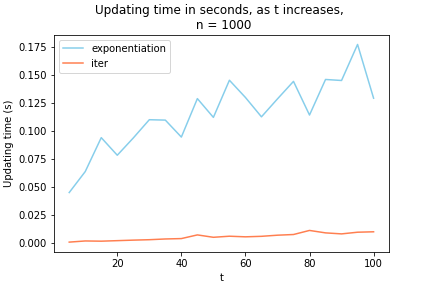
\includegraphics[width=.45\textwidth]{ThesisKI/Images/UpdatingTimeDense.png} }}%
    \qquad
    \subfloat[\centering Sparse Matrix]{{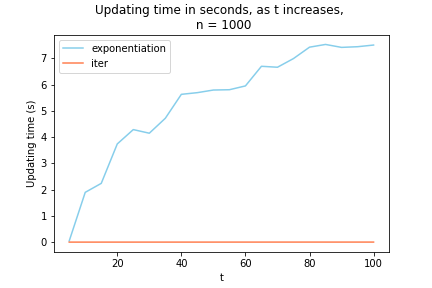
\includegraphics[width=.45\textwidth]{ThesisKI/Images/UpdatingTimeSparse.png} }}%
    \caption{Updating time}%
    \label{update:time}%
\end{figure}

Therefore the iterative method was implemented, in order to significantly speed the updating process. Furthermore, this also allows for saving all intermediate belief vectors, providing insight in the rate of convergence of the network.

However, as shown by \cite{degroot1974concensus}, the convergent belief can also be computed directly, using the eigenvector of the interaction matrix, $\T$, corresponding to $\lambda=1$. Therefore another function was made for those cases where only the convergent belief is of interest. This function gives only the convergent opinion of the network.

\subsection{$\varepsilon$-DeGroot}
\subsubsection{Standard}

The second updating rule that can be sued to converge a network is the $\varepsilon$-DeGroot variation mentioned in section [REF]\todo{ref naar section $\varepsilon$}. The general framework is the same as for standard DeGroot method: repeatedly apply the updating rule until the beliefs stop changing. However, to converge a network using this method a slight modification is necessary. First of all under the $\varepsilon$-DeGroot dynamics the belief vectors do not adhere to the standard notion of convergence as under regular DeGroot dynamics, rather, using this updating rule results in what \cite{amir2021robust} describe as \textit{alternating convergence}. That is to say, rather than one single convergent belief vector, there are two convergent belief vectors, between which the agents alternate.
Therefore, using the same condition for convergence as regular DeGroot mechanics will result in an infinite loop, as the belief vectors will alternate, ensuring there will always be a difference between the beliefs at $t$ and $t-1$. To this end, the convergence condition is changed somewhat. Rather than comparing the beliefs between $t$ and $t-1$ only, the belief vectors are compared between $t$ and $t-2$, to check whether their difference is 0, or near enough. This is also done for the beliefs at $t-1$ and $t-3$ to check whether both of the alternating belief vector have converged. As long as convergence has not occurred for both belief vectors the agents the process keeps repeating.

\subsubsection{Alternative}

The alternate $\varepsilon$-DeGroot dynamics work similarly to the standard $\varepsilon$-DeGroot updating rule, as described in [REF] \todo{ref naar alt $\varepsilon$}. Similarly, it also displays \textit{alternating} convergence, rather than the more standard notion of converge. Therefore, in order to properly detect when the network has converged the same conditions for converge are used as with the standard $\varepsilon$-DeGroot mechanics.

\subsection{Private Belief}

Another updating rule implemented allowed each individual agent to account for a private, constant, belief when updating their opinion. In the chosen implementation this private belief was chosen to be the initial belief at time $t=0$. This way agents will always place some amount of weight on their initial belief. The weight placed on this initial belief is specified by the parameter $\alpha \in [0, 1]$. Converging a network using this updating rule, follows the same process as regular DeGroot mechanics, i.e. repeatedly applying the updating rule until the belief vector no longer changes between iterations. As this updating method results in the more standard notion of convergence, opposed to \textit{alternating} convergence, no further modifications to the convergence procedure were required.

\subsection{Threshold}

Another, minor, modification to the regular DeGroot updating mechanics imposes a threshold on the updating rule, ensuring that agents do not drastically change their opinion in a single updating step. Whenever an agent changes their opinion between two time-steps they can change their opinion by no more than the given threshold, effectively limiting how volatile an agents opinion is, simulating a hesitancy in rapid, drastic, changes in opinion.

\subsection{Variable Weights}

\section{Non-cooperative Agents}

Several implementations for the non-cooperative agents in the network were considered.

The first thought was to give each agent a small chance to become non-cooperative when creating their respective links. However, this would easily disrupt the connectedness of the generated network, as the non-cooperative agents, by definition do not have any incoming links. Any agents added after would lose the guarantee of connectedness, as the non-cooperative agents break the chains. However, this could be worked around by accounting for the already present non-cooperative agents when generating the guaranteed links. However, a more severe downside is how this removes the ability to easily switch between a cooperative and non-cooperative network. Furthermore, this method would not guarantee a non-cooperative agent in the network at any given size, as each agent would randomly be chosen to be non-cooperative.

Therefore, in order to prevent these issues from occurring a different method was chosen. The most important difference is that, where the previous method would choose the non-cooperative agents randomly \textit{during} the network generation process, this method would add them to network \textit{after} the cooperative agents. Furthermore, instead of each agent having a random chance to be non-cooperative, a fixed amount of non-cooperative agents, specified beforehand, is added to the network. For each non-cooperative agent a number of links, to random agents, is created. In order to ensure the presence of these non-cooperative agents in networks of every size the first non-cooperative agents sends a link to the first agent in the network, the second agent sends a link to the second agent in the network, etc. The degree of these non-cooperative agents is determined by the average degree of all cooperative agents in the network, to ensure that they do not have an undue amount of influence over the other agents, or significantly less. Then, after the agents who will receive a link from those non-cooperative agents are determined, their respective indeces are all stored in a list. In order to actually add the non-cooperative agents to the network the network of the desired size is simply taken, and for each non-cooperative agent an empty, i.e. containing only zeroes, is added to the interaction matrix. These rows represent the lack of incoming links to the non-cooperative agents, ensuring they will not update their opinion between time-steps. Subsequently, a column, containing the links to the previously determined agents, is added for each non-cooperative agent. In order then grow the same network by one agent, the original interaction is simply taken again, with the desired amount of additional agents, after which the non-cooperative agents are added anew. As the agents to receive a link from the non-cooperative agents were predetermined, this ensures the structure of the network is retained as the network grows and the non-cooperative agents and their links do not have to be generated from scratch at every network size.

\newpage
\section{Appendix}
\subsection{Proof of (strong) connectedness}

\textbf{Base Case:} \newline
Let $S_1$ be a random social network of 1 agent, generated using the method described in \ref{generation:random}.
S is guaranteed to be fully connected, as the first agent in a network always receives a self-link.\newline

\textbf{Induction Hypothesis:}\newline
Let $S_n$ be an arbitrary, strongly connected, randomly generated network, obtained by the method described in \ref{generation:random}. Now let $S_{n+1}$ be the network that is obtained by growing the network $S_n$ by one agent. We now want to prove that if $S_{n+1}$ is grown from $S_n$ using the method from \ref{generation:random}, $S_{n+1}$ is also strongly connected.\newline

To grow the network $S_n$ by one agent, the agent $n+1$ is added to the network, with two guaranteed links, one incoming and one outgoing. Let the $i$ and $j$ be the arbitrary agents involved in these links, respectively. By the generation procedure outlined in \ref{generation:random}, these agents are guaranteed to be present in $S_n$. However, by our induction hypothesis we now that $S_n$ is strongly connected, therefore there exists a directed path from $i$ and $j$ to any other agent in the network. Therefore, as agent $n+1$ has an incoming link from agent $i$, there exists an incoming path from any agent in the network to $n+1$, and, furthermore, as $n+1$ has an outgoing link to agent $j$, there also exists an outgoing path to any agent in the network. Therefore, as there exists a directed path to any agent in the network from agent $n+1$, $S_{n+1}$ must be strongly connected.\newline
Therefore, as $S_n$ and $S_{n+1}$ were arbitrary networks, it must be the case that any network generated using this method must be strongly connected.\newline

\bibliographystyle{apalike}
\bibliography{references.bib}

\newpage
\end{document}